\begin{apendicesenv}
  
  \chapter{Processo de Engenharia de Requisitos}
  
    \begin{figure}[!htbp]
      \centering
      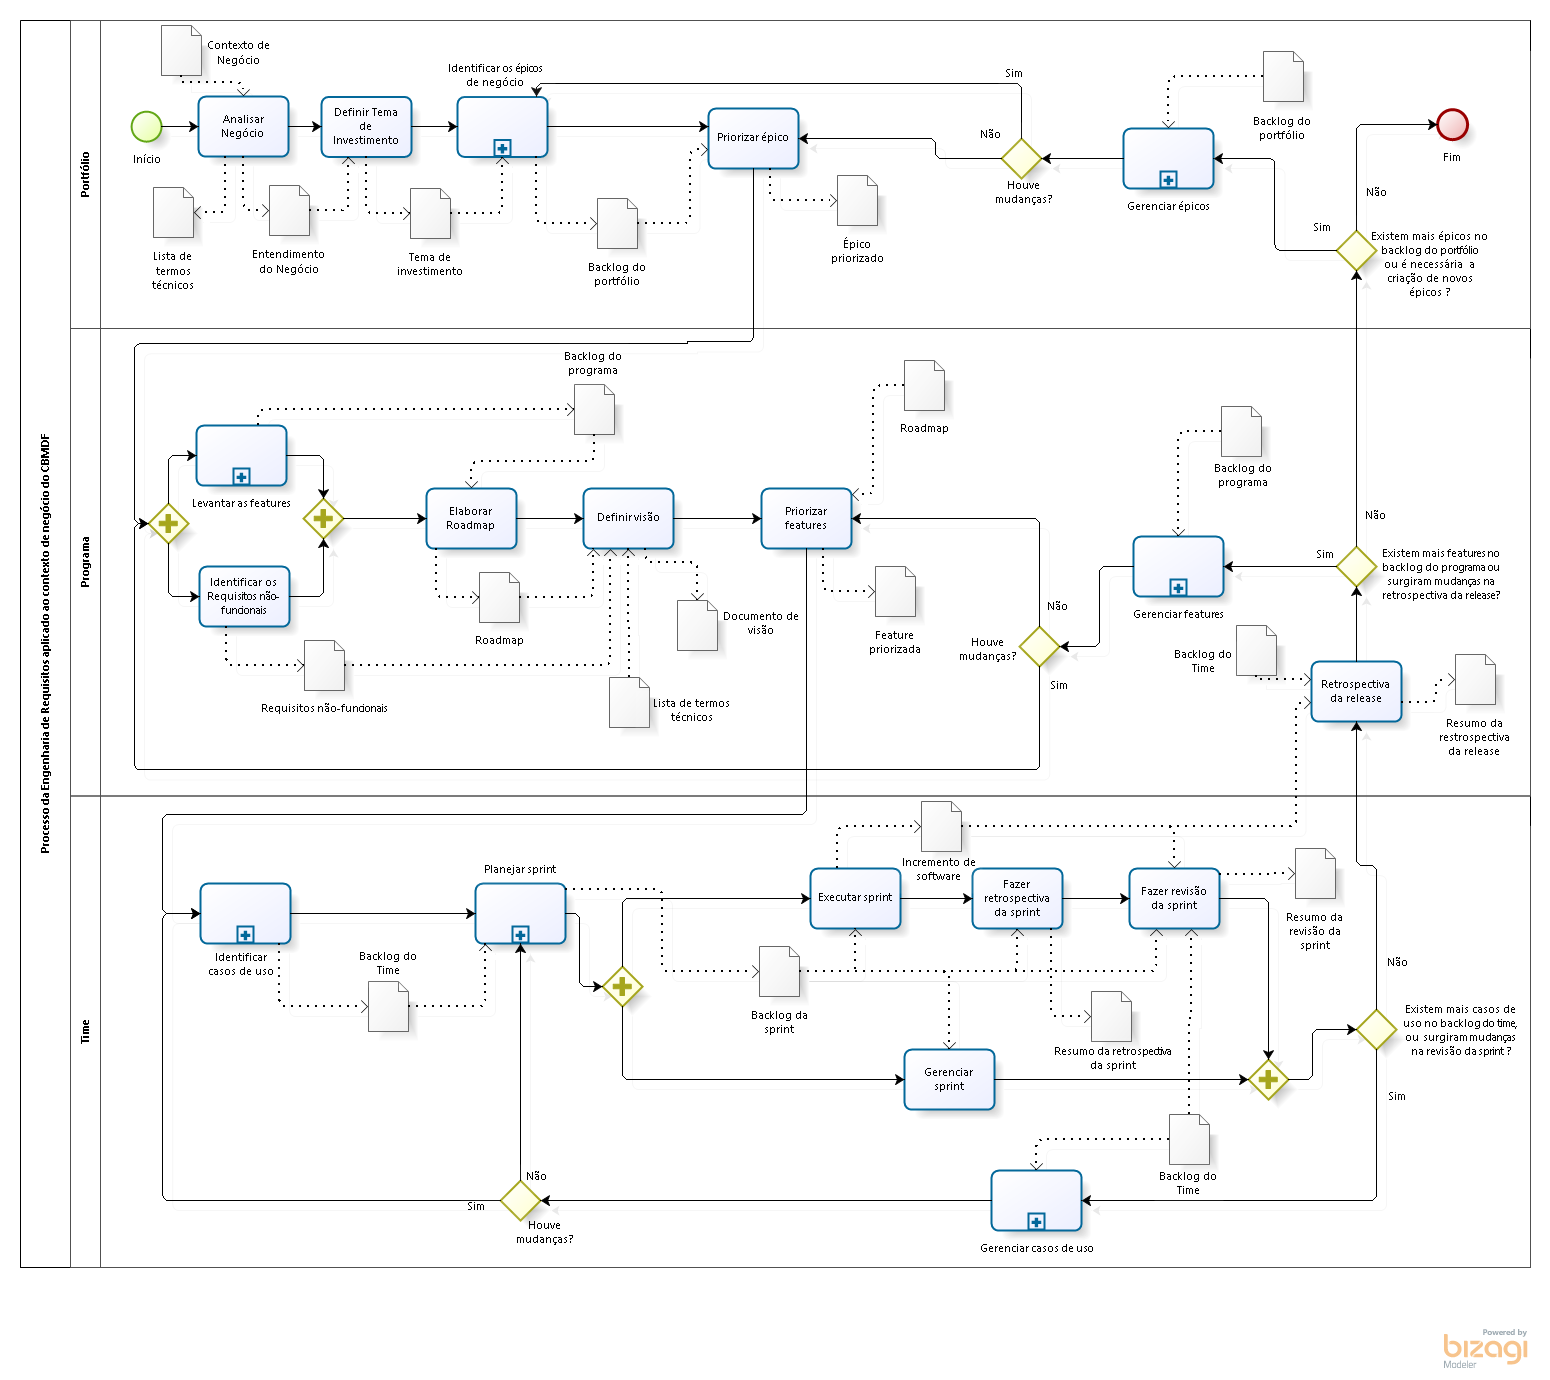
\includegraphics[scale=0.46, angle = 90]{editaveis/figuras/project_big_picture}
      \caption[Modelo do processo de Engenharia de Requisitos]
	  {Modelo do processo de Engenharia de Requisitos: \textit{Big Picture} do projeto.}
      \label{project_big_picture}
    \end{figure}
  
  \chapter{Documento de visão}
	{\centering
	\textbf{Corpo de Bombeiros Militar do Distrito Federal}

	\textbf{Documento de visão para o sistema de gerenciamento de viaturas}

	\textbf{2015}

	}
	\textbf{Histórico de Revisões}
	\begin{table}[h]
	\centering
	\label{my-label}
	\begin{tabular}{|l|l|l|l|}
	\hline
	Data & Revisão & Descrição & Autor \\ \hline
	14/06/2015 & 1.0 & Versão Inicial & João Paulo \\ \hline
	     &         &           &       \\ \hline
	     &         &           &       \\ \hline
	\end{tabular}
	\caption{Histórico de Revisões}
	\end{table}
  
	\section{Introdução}
		\subsection{Propósito}
Este documento define as estratégias utilizadas para nortear o desenvolvimento do projeto, as necessidades do usuário e envolvidos no projeto,
		\subsection{Resumo da solução}
A solução se apresenta sob a forma de uma aplicação que funcionará na intranet do Corpo de Bombeiros Militar do Distrito Federal, e fornecerá subsídios para o correto gerenciamento das viaturas e pessoal relacionado à esse contexto. A aplicação será desenvolvida a partir das necessidades do cliente, sem conexão com um sistema legado.
		\subsection{Referências}
Adicionar Referências
	\section{Descrição do Usuário}
		\subsection{\textit{User Personas}}
Definir User Personas?
		\subsection{Ambiente de Usuário}
Os usuários são funcionários do Corpo de Bombeiros Militar do Distrito Federal e utilizarão o sistema nos batalhões e Unidades.
		\subsection{Principais necessidades do Usuário}
Para o usuário é primordial organizar e automatizar a gestão do contexto de viaturas e motoristas, desde o Departamento de Gestão Veicular até o controle de viaturas e motoristas nas unidades.
	\section{\textit{Stakeholders}}
Definir Stakeholders?
	\section{Resumo do Produto}
Nesta seção serão definidas características do produto.
		\subsection{Perspectiva do Produto}
Espera-se do produto que melhore a gestão de viaturas e motoristas no CBM-DF, facilitando consultas, relatórios, verificações e utilização.
		\subsection{Intenção do Produto}
O sistema de gerenciamento automatizará as atividades que hoje são feitas à mão e são arquivadas sob forma de planilhas eletrônicas. Os usuários do DGV e Unidades utilizarão o sistema afim de automatizar suas atividades.
		\subsection{Resumo das Capacidades}
O sistema de Gerenciamento de Viaturas e Motoristas do CBM-DF permitirá o gerenciamento de viaturas, criando viaturas nos sistemas, alocando viaturas às unidades e modificando os estados das viaturas. Também serão gerenciados os motoristas, adicionando os mesmo no sistema, modificando dados do motorista, alocando motoristas em escalas e em viaturas.
		\subsection{Suposições e Dependências}
A
		\subsection{Preços e Custos}
A
	\section{\textit{Features} do Produto}
A
		\subsection{Feature 1}
A
		\subsection{Feature 2}
A
		\subsection{Feature 3}
A
	\section{Exemplos de Caso de uso}
A
	\section{Requisitos não-funcionais}		
A
		\subsection{RNF 1}
A
		\subsection{RNF 2}
A
		\subsection{RNF 3}
A
			\subsubsection{Padrões de aplicação}
A
			\subsubsection{Licença, segurança e aplicação}
A
	\section{Documentação dos Requisitos}
A
		\subsection{Manual do Usuário}
A
		\subsection{Ajuda Online}
A
		\subsection{Guia de instalação, configuração e arquivo \textit{ReadMe}}
A
		\subsection{Rotulagem dos requisitos e Empacotamentos}
A
		\subsection{Glossário}
Neste item definimos termos a fim de tornar comum o entendimento dos envolvidos.
\begin{itemize}
 \item \textit{Stakeholder}: Envolvido com a produção,utilização ou gerenciamento do projeto.
 \item CBM-DF: Corpo de Bombeiros Militar do Distrito Federal.
 \item DGV: Departamento de Gestão Veicular.
 \item Chamado: Demanda criada por uma ligação de telefone e passada pela central para alguma unidade.
 \item Missão: Atividade dos bombeiros das unidades.

\end{itemize}



\end{apendicesenv}
